\chapter{Metoder}
Afsnittet indeholder en beskrivelse af hvilke metoder, der er blevet anvendt til udarbejdelse af denne mini-MTV i forhold til de fire MTV aspekter: Teknologi, Organisation, Patient og Økonomi.

Overordnet set er der blevet gennemført en litteratursøgning og -vurdering på baggrund af en søgeprotokol, se Bilag 11. Protokollen er udarbejdet ud fra specifikke søgestrategier, hvor der er søgt på engelsk og dansk. De specifikke søgeord er medtaget som dokumentation. Der er søgt i følgende databaser: Embase, PubMed, Google Scholar, Cochrane og Engineering Village. 

Generelt har det været et problem at finde videnskabelige artikler til alle afsnit i rapporten undtagen til Organisation. Videnskabelige artikler omhandlende arbejdsskader har været relativt nemme at fremsøge, dog har det ikke været muligt at finde relevant litteratur til Økonomi. Endvidere har det været nødvendigt at hente oplysninger gennem semi-strukturerede interviews for at få et indblik i organisationen og patientoplevelsen på HEH og RMV, samt teknologien bag Ultralyds Robotarmen. Semi-strukturerede interviews blev benyttet for at have samme udgangspunkt til begge interviews, så oplysningerne kunne sammenlignes. 
Interviews er blevet afholdt med afdelingssygeplejerske Tina Arnbjørn og tre sonografer fra HEH og  afdelingssygeplejerske Karen Marie Goul og en sonograf fra RMV. Efter interviews blev flere scanninger, af forskellige typer, overværet. 
Til at underbygge problemstillingen omkring arbejdsgener suppleres der med videnskabelige artikler.   

De fremsøgte artikler er blevet sorteret ud fra inklusions- og eksklusionskriterier, se figur \ref{InklusionEksklusion}. 

\begin{figure}[H]\centering
	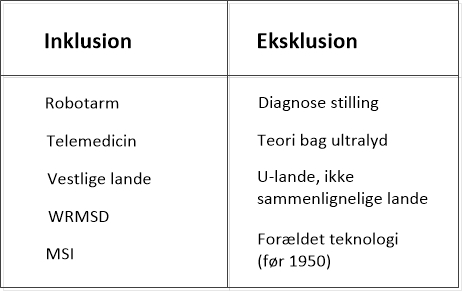
\includegraphics[width = 0.6\textwidth]{Figurer/InklusionEksklusion}
	\caption{Inklusion- og eksklusionkriterier ved litteratursøgning.}
	\label{InklusionEksklusion}
\end{figure}

Dermed er artikler omhandlende scanning af gravide, scanning af hjertet, robotarm og arbejdsskader hos sonografer inkluderet i mini-MTV'en.

Udover ovenstående litteratur er der søgt efter ikke-videnskabelig litteratur for at opnå en forståelse for opbygningen af sonograf uddannelse, ultralydsscanning og ad hoc emner for at komme ind i problemstillingen. 

\section{Teknologi}
Dataindsamling til Teknologi er sket via antagelser fra CEO Søren Pallesen, Robotic Ultrasound ApS, se Bilag 6, produktspecifikationer, se Bilag 1, Bilag 2 og Bilag 3, samt information fra interview af sonografer på HEH og RVM, se Bilag 4 og Bilag 5. Det var ønsket, at dataindsamlingen til Teknologi var sket via videnskabelige artikler, der underbyggede brugen af Ultralyds Robotarmen til scanninger af gravide.
Endvidere skulle videnskabelige artikler have skabt evidens for sikkerhedsindstillinger og tekniske specifikationer til sammenholdning med Søren Pallesens antagelser.\\
Oplysninger fra interview belyser det eksisterende udstyr på afdelingerne. Afsnittet belyser Ultralyds Robotarmens anvendelsesområder, specifikationer, effektivitet, samt sikkerhedsindstillinger.

\section{Organisation}
Dataindsamling til Organisation er sket via kontakt til aktører gennem interviews på HEH og RMV, samt videnskadelige artikler. Analysen bag Organisation bygger på dataindsamling fra to kliniske afdelinger, HEH og RMV, derfor vil dens generaliserbarhed potentielt være begrænset. Resultatet heraf kan derved ikke nødvendigvis anvendes på lignende hospitalsafdelinger i Danmark. \\
De videnskabelige artikler benyttes til at klarlægge omfanget af problemstillingen og opnå en forståelse for, hvilke akavede arbejdsstillinger, der er tale om. \\
Den primære tanke til dataindsamling omkring sonografernes arbejdsgange og scanningsproducere var udarbejdelse af et spørgeskema, der skulle sendes til sonograferne på de enkelte afdelinger, se Bilag 13. Derefter var tanken, at data fra spørgeskemaerne skulle sammenlignes med oplysninger fra interviews med afdelingssygeplejersker. På denne måde kunne det testes om informationerne stemte overens. Eftersom der var for få sonografer på RMV og HEH til at give en valid svarprocent, blev spørgeskemaet fravalgt. \\
Dermed er interviews endt med at blive brugt til at klarlægge sonografers arbejdsgange og de enkelte afdelingers organisering, se Bilag 4 og Bilag 5. 

Afsnittet belyser betydningen ved implementeringen af den nye teknologi for afdelingen som organisation, samt mulige ændringer for personalet. Derudover er Leavitts organisationsmodel blevet benyttet til at beskrive de fire organisatoriske hovedelementer \cite{Leavitt}.

\section{Patient}
Patient bygger på oplysninger fra interviews med sonografer på HEH og RMV, samt etik-delen af kurset ST4MTV-01. Derudover er de fem patientaspekter: sociale, økonomiske, etiske, individuelle og kommunikative forhold blevet benyttet til at belyse den pågældende teknologi og de faktorer, der har betydning for sonografers og patientens hverdagsliv \cite{Leavitt}.\\ 
Den etiske vurdering tager udgangspunkt i problemstillinger, der påvirker gravide og sonografer. Disse problemstillinger omhandler de professionsetiske principper, som den etiske vurdering er baseret på \cite{Husted} \cite{Etiskehjul}.

\section{Økonomi}
Den økonomiske dataindsamling er primært sket på baggrund af kontakt til aktører via telefon, interview og mailkorrespondance. Derefter er dokumenter og andre skriftlige kilder afsøgt, typisk ved at holde dem op mod mundtlige kilder. Vurderingen er udarbejdet med udgangspunkt i omkostningsminimeringsanalyse (CMA) \cite{Leavitt}. Her er der blevet opdelt i to scenarier, det nuværende og det fremtidige. Det nuværende scenarie er en ultralyds scanningsstue, og det fremtidige er en scanningsstue med Ultralyds Robotarmen. For begge scenarier er der medtaget indirekte omkostninger, som ikke har været mulige at prissætte. De økonomiske beregninger indeholder flere af projektgruppens antagelser, hvor det ikke har været muligt at finde videnskabelige artikler med tilstrækkelig økonomisk evidens. Annuitetsformlen er brugt til at beregne afskrivning af Ultralyds Robotarmen \ref{Formler}. 